\documentclass[notes,10pt, aspectratio=169]{beamer}

\usepackage{pgfpages}
% These slides also contain speaker notes. You can print just the slides,
% just the notes, or both, depending on the setting below. Comment out the want
% you want.
\setbeameroption{hide notes} % Only slide
%\setbeameroption{show only notes} % Only notes
%\setbeameroption{show notes on second screen=right} % Both

\usepackage{helvet}
\usepackage[default]{lato}
\usepackage{array}
\usepackage{eurosym}
\usepackage{setspace}
\usepackage{animate}
\usepackage{multicol}
\usepackage{breqn}
\usepackage{subcaption}
\usepackage{caption}
\captionsetup{font=scriptsize, justification=raggedright,singlelinecheck=false}
\usepackage[export]{adjustbox}
\usepackage[scale=2]{ccicons}
\usepackage{tikz}
\newenvironment{wideitemize}{\itemize\addtolength{\itemsep}{10pt}}{\enditemize}
\usepackage{natbib}

\usepackage{tikz}
\usepackage{verbatim}
\setbeamertemplate{note page}{\pagecolor{yellow!5}\insertnote}
\usepackage{amsmath}
%\usepackage{mathpazo}
\usepackage{hyperref}
\usepackage{lipsum}
\usepackage{multimedia}
\usepackage{multirow}
\usepackage{graphicx}
\usepackage{dcolumn}
\usepackage{bbm}
\newcolumntype{d}[0]{D{.}{.}{5}}

\usepackage{changepage}
\usepackage{appendixnumberbeamer}
% \newcommand{\beginbackup}{
%   \newcounter{framenumbervorappendix}
%   \setcounter{framenumbervorappendix}{\value{framenumber}}
%   \setbeamertemplate{footline}
%   {
%      \leavevmode%
%      \hline
%      box{%
%       \begin{beamercolorbox}[wd=\paperwidth,ht=2.25ex,dp=1ex,right]{footlinecolor}%
% %         \insertframenumber  \hspace*{2ex} 
%       \end{beamercolorbox}}%
%      \vskip0pt%
%   }
%  }


\usepackage{minted}   % code prettyfier
\usepackage{xsavebox} % file-size-efficient saveboxes
\usepackage{animate}  % for animated scrolling
\usepackage{MnSymbol} % \triangle, \triangledown for scroll buttons
\usepackage{media9}   % buttons

%%%%%%%%%%%%%%%%%%%%%%%%%%%%%%%%%%%%%%%%%%%%%%%%%%%%%%%%%%%%%%%%%%%%%%%%%%%%%%
% \smoothScroll[<animate opts>]    % autoplay,loop,... (see: texdoc animate)
%              {<xsavebox id>}
%              {<viewport height>}
%              {<steps>}           % scrolling granularity
%              {<steps per sec>}   % while playing; >25 doesn't make sense
%%%%%%%%%%%%%%%%%%%%%%%%%%%%%%%%%%%%%%%%%%%%%%%%%%%%%%%%%%%%%%%%%%%%%%%%%%%%%%
\newcommand\smoothScroll[5][]{%
  \savebox\myMeasBox{\xusebox{#2}}%
  \edef\mywd{\the\wd\myMeasBox}%
  \edef\myht{\the\ht\myMeasBox}%
  \edef\mytht{\the\dimexpr\ht\myMeasBox+\dp\myMeasBox\relax}%
  \edef\portht{\the\dimexpr#3\relax}%
  \begin{animateinline}[#1,label={#2},width=\mywd,height=\portht]{#5}%
    \multiframe{#4}{%
      dRaiseLen=\the\dimexpr-\myht+\portht\relax+\the\dimexpr(\mytht-\portht)/%
                \numexpr#4-1\relax\relax
    }{%
      \begin{minipage}[b][\portht][b]{\mywd}%
        \raisebox{\dRaiseLen}[0pt][0pt]{\xusebox{#2}}%
      \end{minipage}%
    }%
  \end{animateinline}%
}
\newsavebox\myMeasBox % for measuring purposes
%%%%%%%%%%%%%%%%%%%%%%%%%%%%%%%%%%%%%%%%%%%%%%%%%%%%%%%%%%%%%%%%%%%%%%%%%%%%%%

%%%%%%%%%%%%%%%%%%%%%%%%%%%%%%%%%%%%%%%%%%%%%%%%%%%%%%%%%%%%%%%%%%%%%%%%%%%%%%
%% \topScrollButton{<xsavebox id>}
%%%%%%%%%%%%%%%%%%%%%%%%%%%%%%%%%%%%%%%%%%%%%%%%%%%%%%%%%%%%%%%%%%%%%%%%%%%%%%
\newcommand\topScrollButton[1]{%
  \mediabutton[
    jsaction={
      if(event.shift){anim['#1'].pause();anim['#1'].frameNum=0;}
      else try{anim['#1'].frameNum--}catch(e){}
    }
  ]{\fboxsep=0pt\framebox[\widthof{\xusebox{#1}}][c]{%
    \tiny\strut\raisebox{-0.2\height}{$\triangle\triangle\triangle$}}%
  }%
}  
%%%%%%%%%%%%%%%%%%%%%%%%%%%%%%%%%%%%%%%%%%%%%%%%%%%%%%%%%%%%%%%%%%%%%%%%%%%%%%

%%%%%%%%%%%%%%%%%%%%%%%%%%%%%%%%%%%%%%%%%%%%%%%%%%%%%%%%%%%%%%%%%%%%%%%%%%%%%%
%% \botScrollButton{<xsavebox id>}
%%%%%%%%%%%%%%%%%%%%%%%%%%%%%%%%%%%%%%%%%%%%%%%%%%%%%%%%%%%%%%%%%%%%%%%%%%%%%%
\newcommand\botScrollButton[1]{%
  \mediabutton[
    jsaction={
      if(event.shift){anim['#1'].pause();anim['#1'].frameNum=anim['#1'].numFrames-1;}
      else try{anim['#1'].frameNum++}catch(e){}
    }
  ]{\fboxsep=0pt\framebox[\widthof{\xusebox{#1}}][c]{%
    \tiny\strut\raisebox{0.1\height}{$\triangledown\triangledown\triangledown$}}%
  }%
}  
%%%%%%%%%%%%%%%%%%%%%%%%%%%%%%%%%%%%%%%%%%%%%%%%%%%%%%%%%%%%%%%%%%%%%%%%%%%%%%


 \setbeamertemplate{footline}{
    \hbox{%
    \begin{beamercolorbox}[wd=\paperwidth,ht=3ex,dp=1.5ex,leftskip=2ex,rightskip=2ex]{page footer}%
        %\usebeamerfont{title in head/foot}%
        %\insertshorttitle \hfill
        %\insertsection \hfill
        %\tableofcontents[currentsection] \hfill
        \insertsectionnavigationhorizontal{0.7\paperwidth}{}{} \hfill 
        \insertframenumber{} / \inserttotalframenumber
    \end{beamercolorbox}}%
}
\newcommand{\backupend}{
   \addtocounter{framenumbervorappendix}{-\value{framenumber}}
   \addtocounter{framenumber}{\value{framenumbervorappendix}} 
}


\usepackage{graphicx}
\usepackage[space]{grffile}
\usepackage{booktabs}

% These are my colors -- there are many like them, but these ones are mine.
\definecolor{blue}{RGB}{0,114,178}
\definecolor{red}{RGB}{213,94,0}
\definecolor{yellow}{RGB}{240,228,66}
\definecolor{green}{RGB}{0,158,115}

\setbeamercolor{section in head/foot}{fg=blue}

\useinnertheme[shadow]{rounded}
\setbeamercolor{block title example}{fg=black,bg=orange!50!white}
\setbeamercolor{block body example}{fg=black, bg=orange!30!white}


\hypersetup{
  colorlinks=false,
  linkbordercolor = {white},
  linkcolor = {blue}
}


%% I use a beige off white for my background
\definecolor{MyBackground}{RGB}{255,253,218}

%% Uncomment this if you want to change the background color to something else
%\setbeamercolor{background canvas}{bg=MyBackground}

%% Change the bg color to adjust your transition slide background color!
\newenvironment{transitionframe}{
  \setbeamercolor{background canvas}{bg=yellow}
  \begin{frame}}{
    \end{frame}
}

\setbeamercolor{frametitle}{fg=blue}
\setbeamercolor{title}{fg=black}
%\setbeamertemplate{footline}[frame number]
\setbeamertemplate{navigation symbols}{} 
\setbeamertemplate{itemize items}{-}
\setbeamercolor{itemize item}{fg=blue}
\setbeamercolor{itemize subitem}{fg=blue}
\setbeamercolor{enumerate item}{fg=blue}
\setbeamercolor{enumerate subitem}{fg=blue}
\setbeamercolor{button}{bg=white,fg=blue,}



% If you like road maps, rather than having clutter at the top, have a roadmap show up at the end of each section 
% (and after your introduction)
% Uncomment this is if you want the roadmap!
% \AtBeginSection[]
% {
%    \begin{frame}
%        \frametitle{Roadmap of Talk}
%        \tableofcontents[currentsection]
%    \end{frame}
% }
\setbeamercolor{section in toc}{fg=blue}
\setbeamercolor{subsection in toc}{fg=red}
%\setbeamersize{text margin left=1em,text margin right=1em} 
\setbeamersize{text margin left=0.7cm,text margin right=0.7cm} 


\title[]{\textcolor{blue}{Practice 3:\\OVB and Technological Change}}
\author{25117 - Econometrics}
\institute[shortinst]{Universitat Pompeu Fabra}

\date{October 28th, 2024}

\begin{document}

% Title Slide

\begin{frame}[plain]
\maketitle
\end{frame}


\begin{frame}{Omitted Variable Bias}
Omitted Variable Bias refers to the bias introduced in regression analysis when a relevant variable is left out of the model. This bias can distort the estimated relationships between variables and lead to incorrect conclusions. It can be represented mathematically as follows:
  \[ \hat{\beta}_{\text{biased}} = \beta_{\text{true}} + \frac{{\text{Cov}(X, Z)}}{{\text{Var}(X)}}  \]
  where:
  \begin{itemize}
      \item \(\hat{\beta}_{\text{biased}}\) is the biased estimator.
      \item \(\beta_{\text{true}}\) is the true parameter of interest.
      \item \(X\) is the included variable.
      \item \(Z\) is the omitted variable.
      \item \(\text{Cov}(X, Z)\) is the covariance between \(X\) and \(Z\).
      \item \(\text{Var}(X)\) is the variance of \(X\).
  \end{itemize}
\end{frame}

\begin{frame}{Introduction to Omitted Variable Bias}
\begin{exampleblock}{Question}
    How can omitting important variables affect our analysis?
\end{exampleblock}
\begin{itemize}
  \item Omitted Variable Bias occurs when a relevant variable is not included in a regression model, and this omission can lead to incorrect conclusions.
  \item For example, if we're studying wage changes and we omit the variable "years of education," we might mistakenly attribute wage changes to other factors, resulting in a biased estimate of the impact of omitted variables.
\end{itemize}
\end{frame}


\begin{frame}{Omitted Variable Bias (OVB)}
\begin{exampleblock}{Question}
    What are the two conditions required on $Z$ for omitted variable bias to occur?
\end{exampleblock}

\vspace{1cm}
\begin{center}
\begin{figure}
    \resizebox{.6\linewidth}{!}{%



\tikzset{every picture/.style={line width=0.75pt}} %set default line width to 0.75pt        

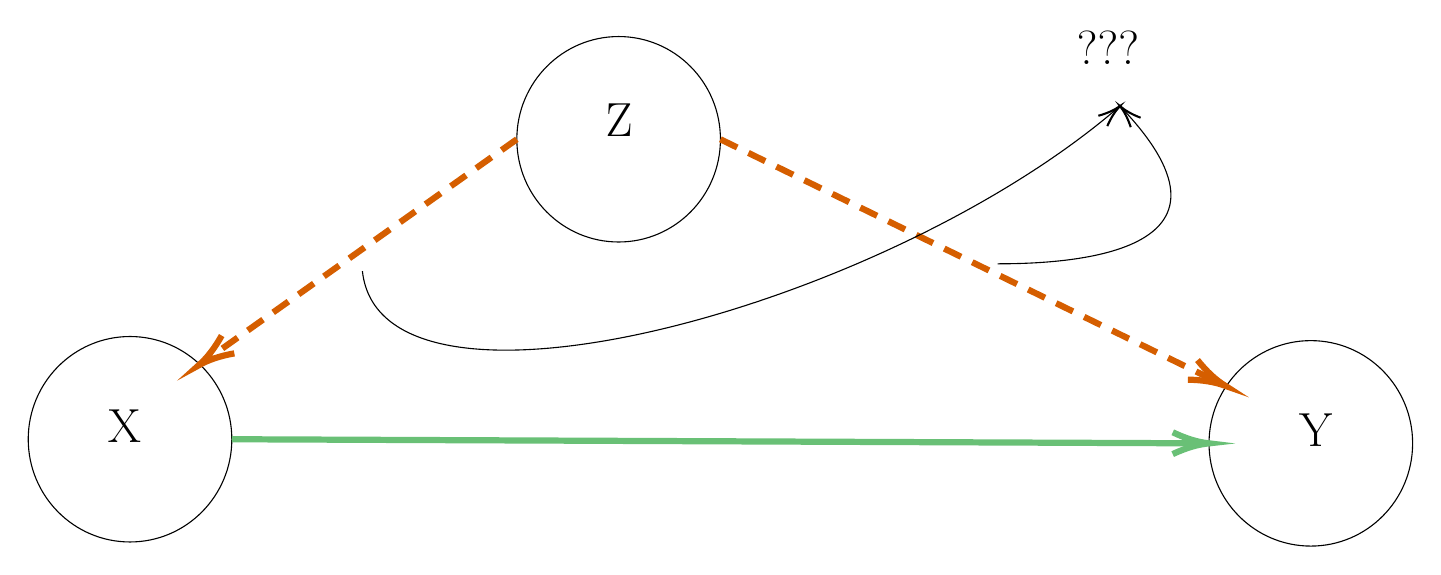
\begin{tikzpicture}[x=0.75pt,y=0.75pt,yscale=-1,xscale=1]
%uncomment if require: \path (0,285); %set diagram left start at 0, and has height of 285

%Shape: Ellipse [id:dp36615011120920427] 
\draw   (254.41,66.5) .. controls (254.41,39.16) and (276.37,17) .. (303.46,17) .. controls (330.54,17) and (352.5,39.16) .. (352.5,66.5) .. controls (352.5,93.83) and (330.54,115.99) .. (303.46,115.99) .. controls (276.37,115.99) and (254.41,93.83) .. (254.41,66.5) -- cycle ;
%Shape: Ellipse [id:dp34906029723118115] 
\draw   (19,211.02) .. controls (19,183.69) and (40.96,161.53) .. (68.04,161.53) .. controls (95.13,161.53) and (117.09,183.69) .. (117.09,211.02) .. controls (117.09,238.36) and (95.13,260.52) .. (68.04,260.52) .. controls (40.96,260.52) and (19,238.36) .. (19,211.02) -- cycle ;
%Shape: Ellipse [id:dp6974919182309072] 
\draw   (587.91,213) .. controls (587.91,185.67) and (609.87,163.51) .. (636.96,163.51) .. controls (664.04,163.51) and (686,185.67) .. (686,213) .. controls (686,240.34) and (664.04,262.5) .. (636.96,262.5) .. controls (609.87,262.5) and (587.91,240.34) .. (587.91,213) -- cycle ;
%Straight Lines [id:da04124970397057681] 
\draw [color={rgb, 255:red, 126; green, 211; blue, 33 }  ,draw opacity=1 ][line width=2.25]    (117.09,211.02) -- (583.91,212.99) ;
\draw [shift={(587.91,213)}, rotate = 180.24] [color={rgb, 255:red, 126; green, 211; blue, 33 }  ,draw opacity=1 ][line width=2.25]    (17.49,-5.26) .. controls (11.12,-2.23) and (5.29,-0.48) .. (0,0) .. controls (5.29,0.48) and (11.12,2.23) .. (17.49,5.26)   ;
%Straight Lines [id:da035209354566531736] 
\draw [color={rgb, 255:red, 255; green, 0; blue, 0 }  ,draw opacity=1 ][line width=2.25]  [dash pattern={on 6.75pt off 4.5pt}]  (254.41,66.5) -- (104.26,173.18) ;
\draw [shift={(101,175.5)}, rotate = 324.6] [color={rgb, 255:red, 255; green, 0; blue, 0 }  ,draw opacity=1 ][line width=2.25]    (17.49,-5.26) .. controls (11.12,-2.23) and (5.29,-0.48) .. (0,0) .. controls (5.29,0.48) and (11.12,2.23) .. (17.49,5.26)   ;
%Straight Lines [id:da19389419961485554] 
\draw [color={rgb, 255:red, 255; green, 0; blue, 0 }  ,draw opacity=1 ][line width=2.25]  [dash pattern={on 6.75pt off 4.5pt}]  (352.5,66.5) -- (592.16,183.53) ;
\draw [shift={(595.76,185.29)}, rotate = 206.03] [color={rgb, 255:red, 255; green, 0; blue, 0 }  ,draw opacity=1 ][line width=2.25]    (17.49,-5.26) .. controls (11.12,-2.23) and (5.29,-0.48) .. (0,0) .. controls (5.29,0.48) and (11.12,2.23) .. (17.49,5.26)   ;
% %Curve Lines [id:da92152652585756] 
\draw    (486,126.5) .. controls (518.84,126.5) and (613.05,122.54) .. (546.02,51.57) ;
\draw [shift={(545,50.5)}, rotate = 46.22] [color={rgb, 255:red, 0; green, 0; blue, 0 }  ][line width=0.75]    (10.93,-3.29) .. controls (6.95,-1.4) and (3.31,-0.3) .. (0,0) .. controls (3.31,0.3) and (6.95,1.4) .. (10.93,3.29)   ;
%Curve Lines [id:da6333756929191379] 
\draw    (180,130) .. controls (189,213) and (432,148.5) .. (545,50.5) ;
\draw [shift={(545,50.5)}, rotate = 139.07] [color={rgb, 255:red, 0; green, 0; blue, 0 }  ][line width=0.75]    (10.93,-3.29) .. controls (6.95,-1.4) and (3.31,-0.3) .. (0,0) .. controls (3.31,0.3) and (6.95,1.4) .. (10.93,3.29)   ;

% Text Node
\draw (56.08,195.51) node [anchor=north west][inner sep=0.75pt]   [align=left] {{\LARGE X}};
% Text Node
\draw (295.97,47.97) node [anchor=north west][inner sep=0.75pt]   [align=left] {{\LARGE Z}};
% Text Node
\draw (630.08,197.51) node [anchor=north west][inner sep=0.75pt]   [align=left] {{\LARGE Y}};
% Text Node
 \draw (523,13) node [anchor=north west][inner sep=0.75pt]  [font=\LARGE] [align=left] {???};


\end{tikzpicture}

}
\end{figure}
\end{center}
\end{frame}


\begin{frame}{Control Variables in Multiple Regression Analysis}
\begin{exampleblock}{Question}
    Why is it important to control for variables that might impact the dependent variable? What do we intend to achieve in these cases?
\end{exampleblock}

\begin{itemize}
  \item It's crucial to control for variables that might impact the dependent variable because doing so helps us isolate the effect of our main independent variable.
  \item For example, when studying wages, we might control for education, experience, and industry to ensure that we're attributing changes in wages specifically to computer use and not to other factors.
\begin{exampleblock}{Question}
    What are ”Control Variables”?
\end{exampleblock}
\end{itemize}
\end{frame}

\begin{frame}{In Practice (1): The Returns to Education Puzzle}
\begin{center}
    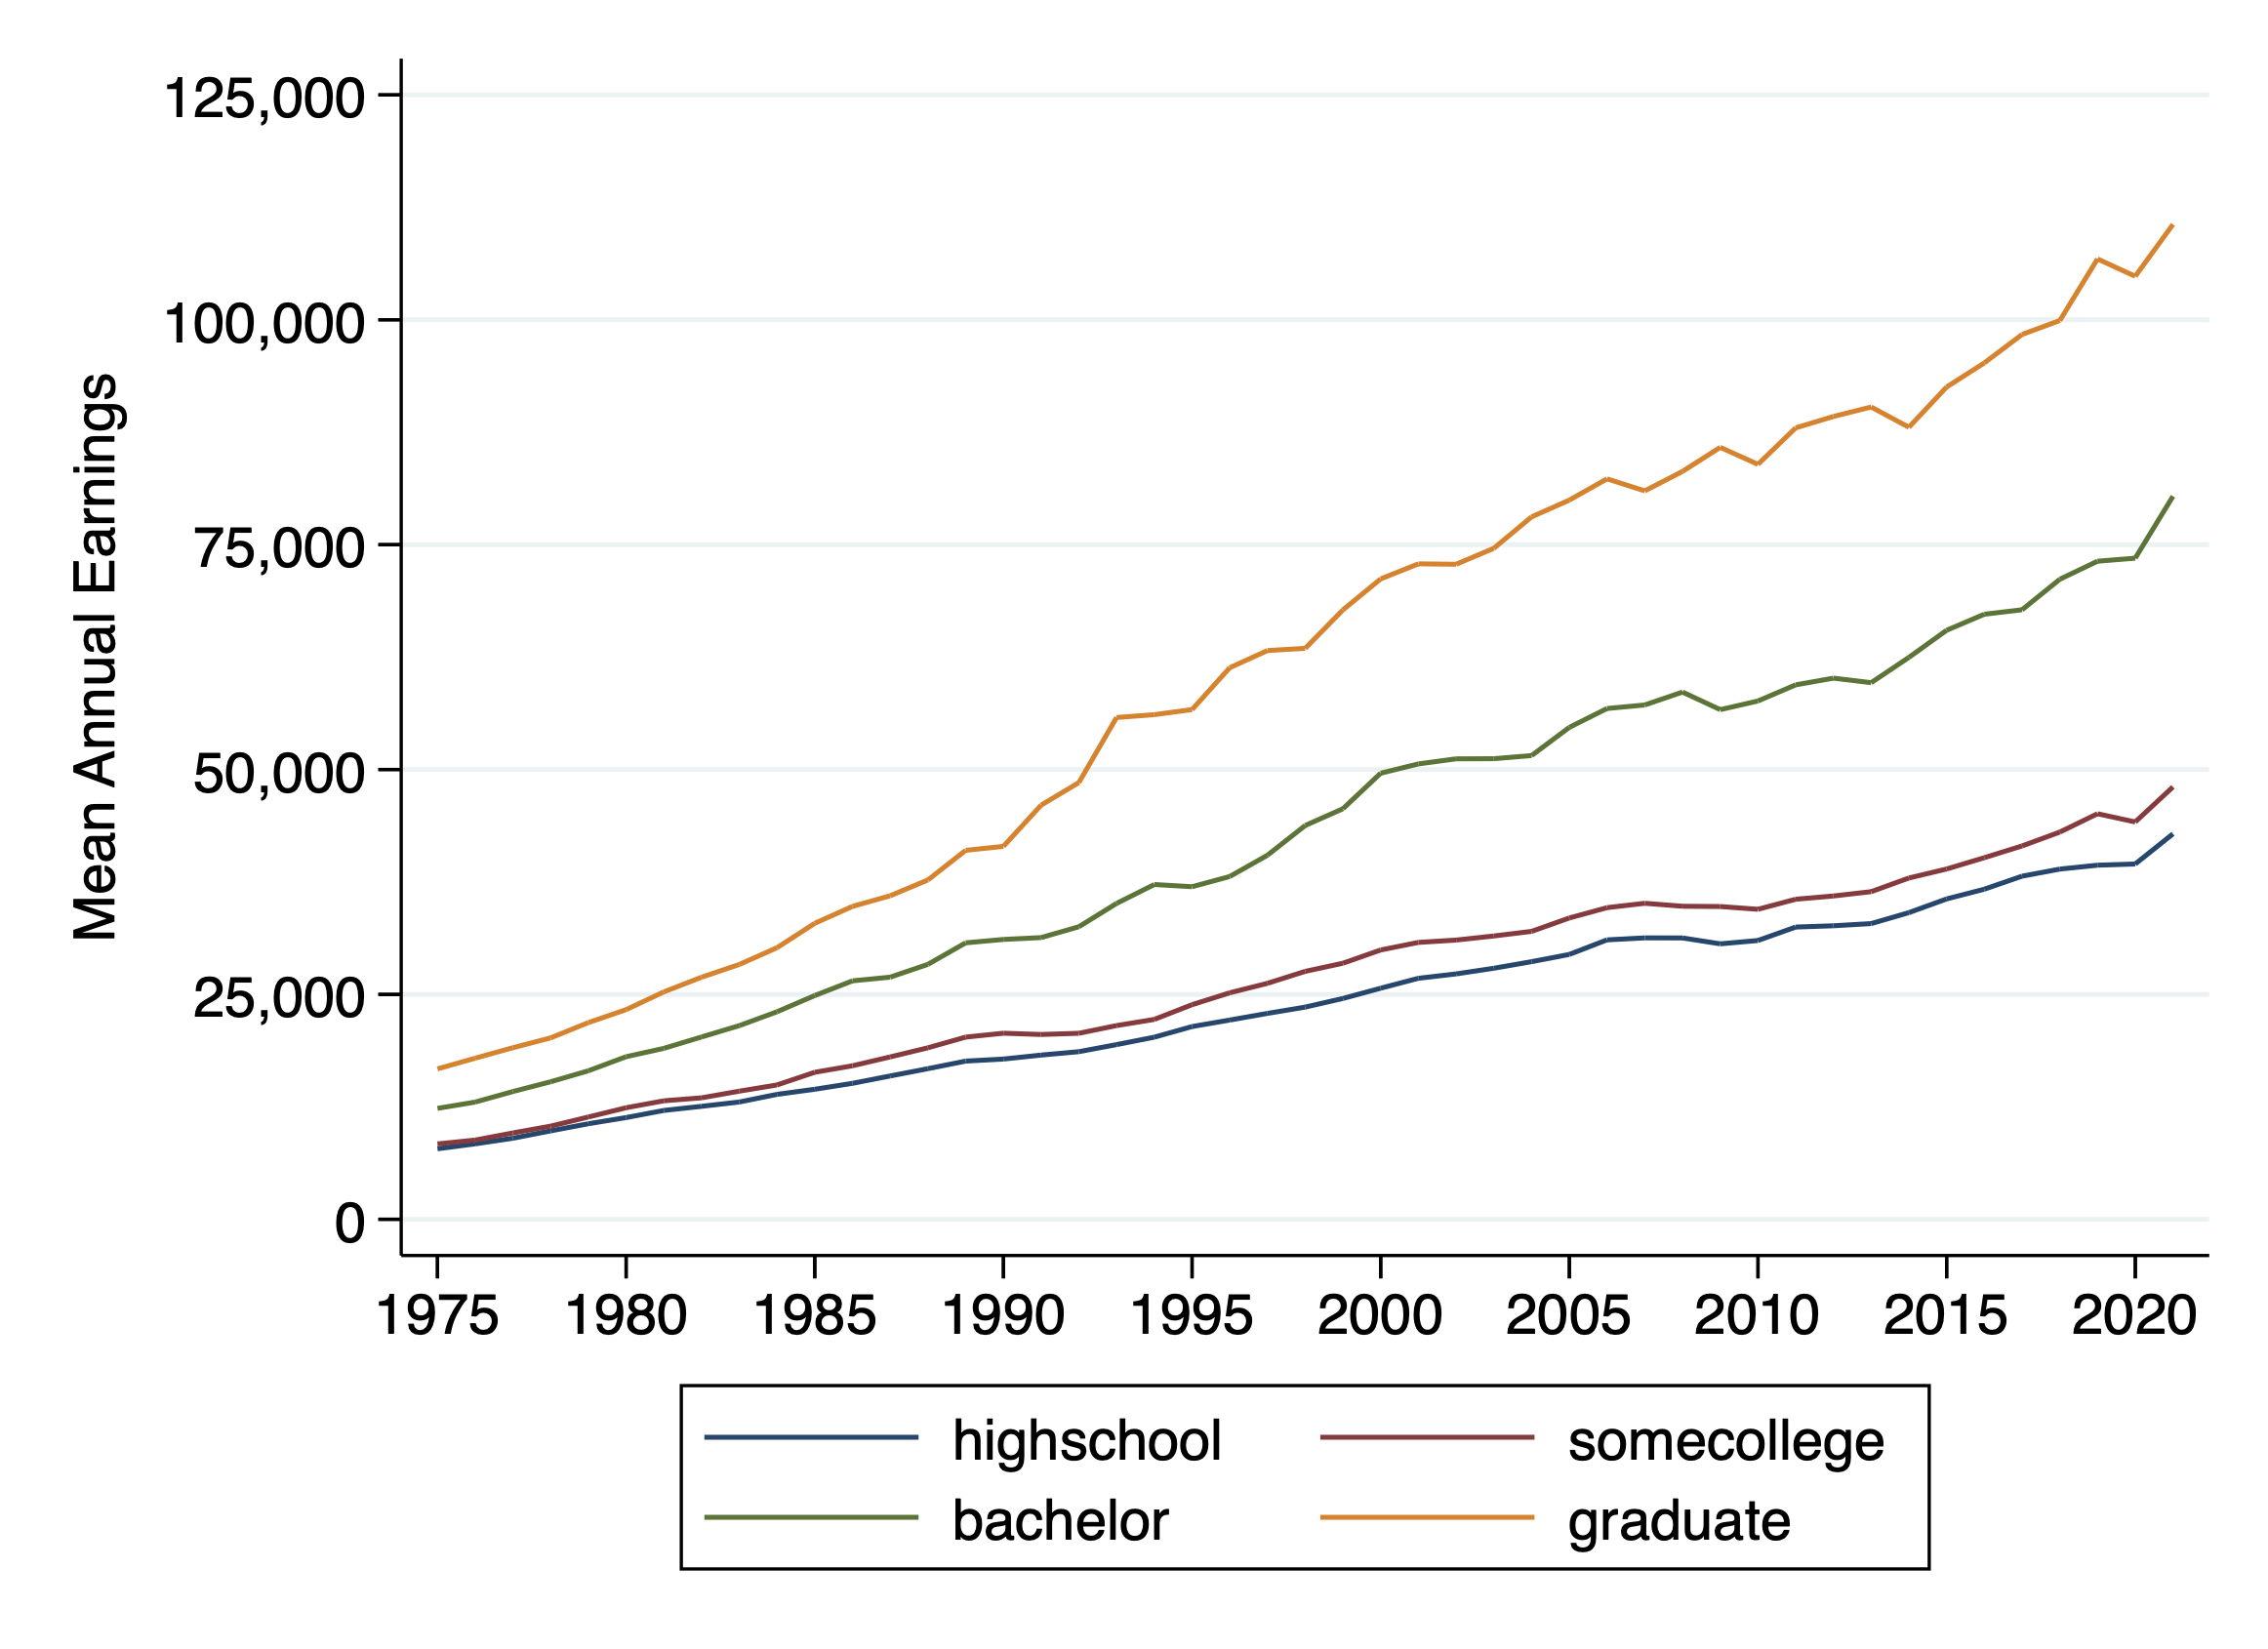
\includegraphics[scale=.27]{images/wage_gap.png}
\end{center}
\end{frame}

\begin{frame}{In Practice (1): The Returns to Education Puzzle}
\begin{center}
    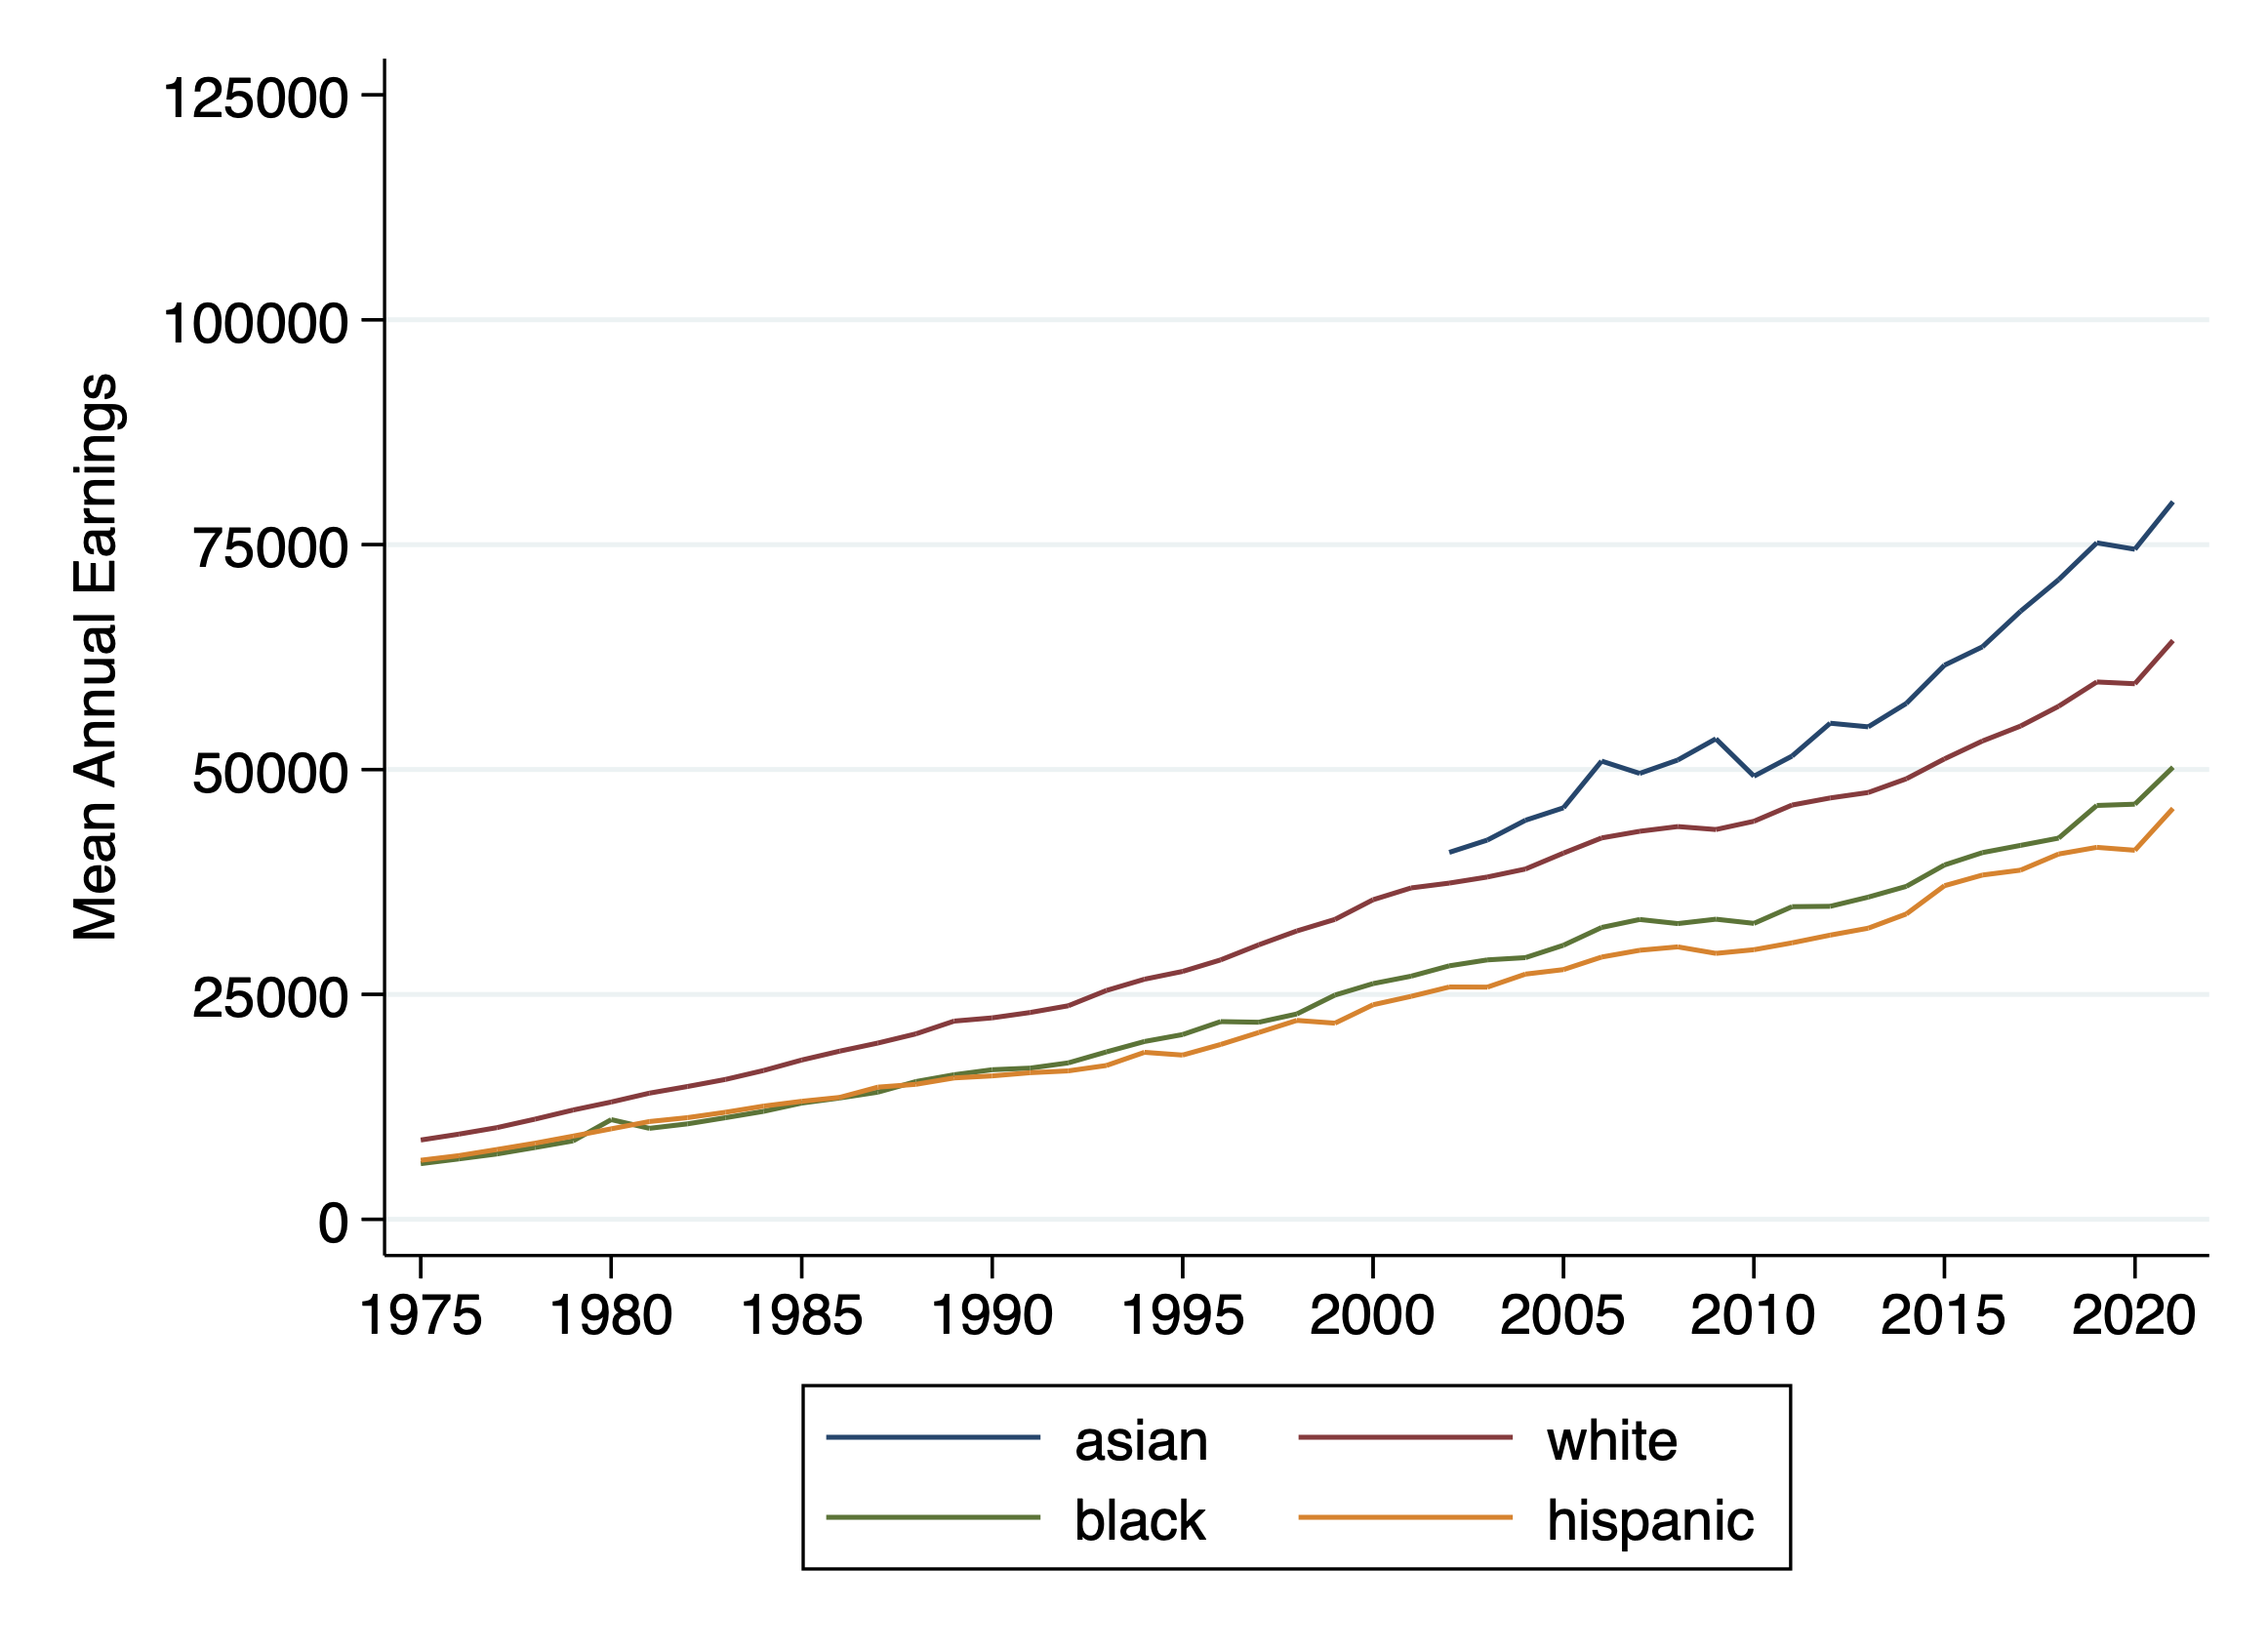
\includegraphics[scale=.27]{images/wage_gap3.png}
\end{center}
\end{frame}

\begin{frame}{In Practice (1): Have Computers Changed the Wage Structure?}
\begin{itemize}
    \item Either
    \begin{enumerate}
        \item increased \textit{international competition} has hurt the position of less-educated workers (less bargaining power) ; and/or
        \item \textit{skill-biased technological change} has affected the relative productivity highly qualified workers
    \end{enumerate}
    \item This is the 80s and it's been 10 years already since the 30-year-old Bill Gates created Microsoft. "Computers" is no longer a word meant to designate a person.
    \item The government charges you to understand the impact of computers on the wage structure
\end{itemize}

    \begin{exampleblock}{Questions}
    \begin{itemize}
        \item What would you expect from the theory?
        \item What would be the gold standard experiment that would allow you to answer this question?
        \item How would you proceed?
        \item In practice, what challenges would you face?
    \end{itemize}
    \end{exampleblock}
\end{frame}



\begin{frame}{In Practice (1): LHS vs RHS}
\begin{itemize}
  \item The previous graphs show the earnings advantage of college graduates and expanding wage differentials based on race. These stylized facts provide insights into the changing wage structure during that period.\\[1em]
  \item ``Wage Structure'' refers to the distribution of wages in an economy and the patterns of wage differentials among different groups of workers. It includes factors such as the earnings gap between high and low-skilled workers or wage disparities based on education or demographics.\\[1em]
  \item The computer revolution can impact wage structure in various ways. For instance, it can lead to higher wages for workers who can effectively use computers, but it may also lead to wage compression for others if they cannot adapt to the technological changes.\\[1em]
  \item The "Computer Revolution" refers to the rapid and transformative changes in the use of computers and technology in various industries and workplaces. It includes the widespread adoption of computers and their impact on work processes and productivity.
\end{itemize}
\end{frame}

\begin{frame}{In Practice (1): Current Population Surveys (CPS)}
\begin{itemize}
  \item \textbf{Definition:} The Current Population Surveys (CPS) are a series of monthly surveys conducted by the U.S. Census Bureau.
  \item \textbf{Purpose:} These surveys are designed to collect a wide range of data on labor force characteristics, economic conditions, and social demographics of the U.S. population.
  \item \textbf{Frequency:} The CPS is conducted on a monthly basis, making it a valuable source of up-to-date information.
  \item \textbf{Sample Size:} The CPS includes a large and diverse sample of households and individuals, making it a representative source of data.
  \item \textbf{Key Features:}
  \begin{itemize}
      \item Provides information on employment, unemployment, and wages.
      \item Collects data on educational attainment, industry, occupation, and more.
      \item Contains supplemental questions on various topics, including computer use in the workplace.
  \end{itemize}
  \item \textbf{Importance:} The CPS is a critical data source as it helps monitor labor market trends and understand the socio-economic landscape of the United States.
\end{itemize}
\end{frame}


\begin{frame}{In Practice (1): Computer Use in the 80s}
\includegraphics<1>[width=\linewidth]{images/kruger01.png}
\includegraphics<2>[width=\linewidth]{images/kruger02.png}
\includegraphics<3>[width=\linewidth]{images/kruger03.png}
\end{frame}

\begin{frame}{In Practice (1): Empirical Strategy}
Krueger (1993)'s empirical question is:\\[.5em]
\begin{quote}
    \textbf{Do employees who use computers at work receive a higher wage as a result of their computer skills?}
\end{quote}\\[1em]
His main specification reads
\begin{equation}
    ln(W_i) = \beta_0 + \beta_1 C_i + \sum_{j=2}^k \beta_j X_{ji} + u_i
\end{equation}

where
\begin{itemize}
    \item $W_i$ is the hourly wage of the $i$th individual
    \item $C_i$ is a dummy variable $=1$ if the $i$th individual uses a computer at work, and 0 otherwise
    \item $X_{ji}$ intends to capture other characteristics of individual $i$ (e.g., educational attainment, etc.)
\end{itemize}

\begin{exampleblock}{Question}
    How do you read this equation? Why include a vector of variables $\mathbf{X}$? Should standard errors be robust to heteroskedasticity? Why?
\end{exampleblock}
\end{frame}



\begin{frame}{In Practice (1): Main Specification (1)}
% typeset code into xsavebox `SomeCode'  
\begin{xlrbox}{SomeCode}%
  \begin{minipage}{\linewidth}%  
    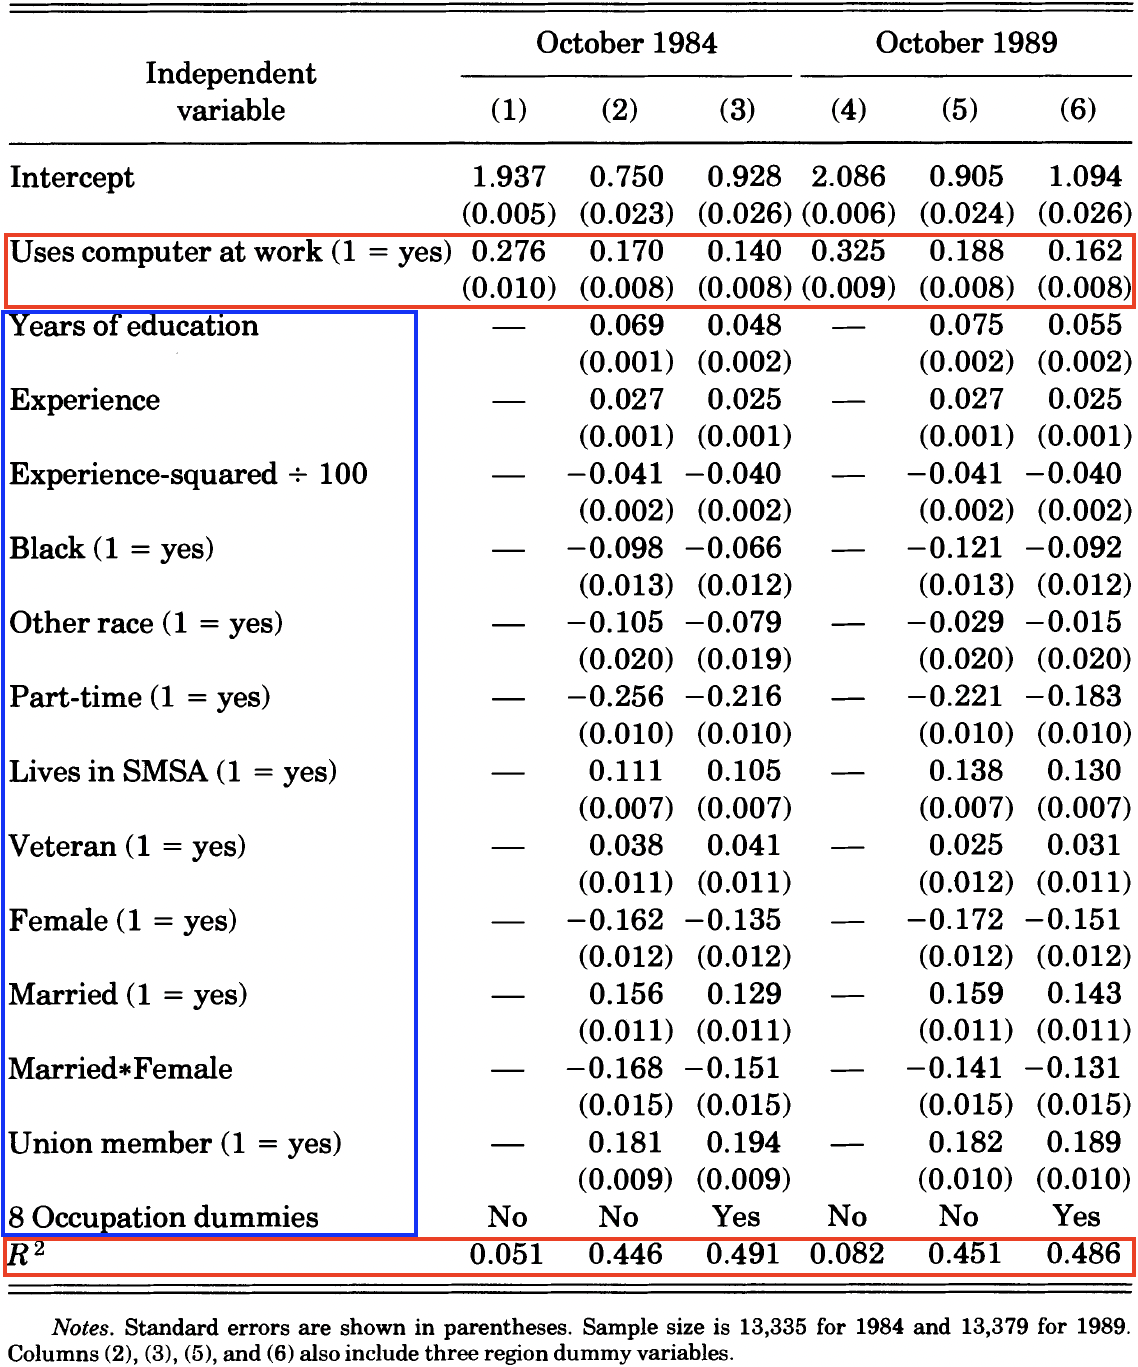
\includegraphics[width=\linewidth]{images/kruger1.png}%
  \end{minipage}%  
\end{xlrbox}%
%
%%%%%%%%%%%%%%%%%%%%%%%%%%%%%%%%%%
\topScrollButton{SomeCode}
%%%%%%%%%%%%%%%%%%%%%%%%%%%%%%%%%%
% scrolling widget
\smoothScroll{SomeCode}{0.75\textheight}{20}{25}
%%%%%%%%%%%%%%%%%%%%%%%%%%%%%%%%%%
\raisebox{2ex}{\botScrollButton{SomeCode}}
%%%%%%%%%%%%%%%%%%%%%%%%%%%%%%%%%%
\end{frame}

\begin{frame}[shrink=5]{In Practice (1): Empirical Strategy Cont'd}
Krueger (1993) is worried that ability might cofound the main effect:\\[.5em]
\begin{quote}
    \textbf{A critical concern in interpreting the OLS regressions reported above is that workers who use computers on the job may be abler workers [...]. The finding that the computer wage differential is attenuated when covariates are included in the OLS regressions suggests that important variables may be omitted that are positively correlated with both computer use and earnings.}
\end{quote}\\[1em]
To capture computer ability, the author estimates the following equation
\begin{equation}
    ln(W_i) = \beta_0 + \beta_1 C_{w,i} + \beta_2 C_{h,i} + \beta_3 C_{hw,i} + \sum_{j=4}^k \beta_j X_{j,i} + u_i
\end{equation}

where
\begin{itemize}
    \item $W_i$ is the hourly wage of the $i$th individual
    \item $C_{w,i}$ is a dummy variable $=1$ if the $i$th individual uses a computer at \textit{work}
    \item $C_{h,i}$ is a dummy variable $=1$ if the $i$th individual uses a computer at \textit{home}
    \item $C_{hw,i}$ is a dummy variable $=1$ if the $i$th individual uses a computer at \textit{home} and at \textit{work}
    \item $X_{ji}$ intends to capture other characteristics of individual $i$ (e.g., educational attainment, etc.)
\end{itemize}

\end{frame}


\begin{frame}{In Practice (1): Controlling for a computer-ability proxy}
\begin{center}
    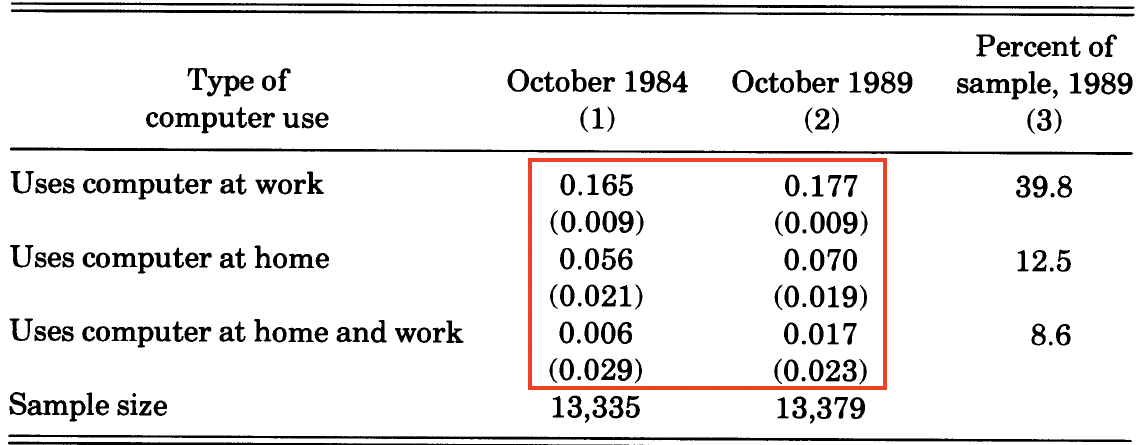
\includegraphics[width=\linewidth]{images/kruger2.png}
\end{center}
\begin{exampleblock}{Question}
    Interpret these coefficients and their associated standard errors. What is the omitted category (comparison group) here?
\end{exampleblock}

\end{frame}


\begin{frame}{In Practice (2): Have Pencils changed the Wage Structure Too?}
\begin{itemize}
  \item The study by Krueger (1993) examines the relationship between computer use on the job and wage differentials.\\[1em]
  \item Krueger's findings suggest that computer users earn 15 to 20 percent more than nonusers after controlling for standard worker attributes.\\[1em]
  \item The study also attempts to address whether this wage differential primarily reflects a "causal" relationship between computer use and wages or is a result of unobserved worker heterogeneity.\\[1em]
  \item Di Nardo and Pischke (1997) replicates Krueger's analysis using data from German workers.\\[1em]
  \item The results in Germany are similar to those found by Krueger in the United States.\\[1em]
  \item The computer wage premium in Germany is estimated to be around 17 percent in 1991.
\end{itemize}
\end{frame}


\begin{frame}{In Practice (2): Have Pencils changed the Wage Structure Too?}
\begin{itemize}
  \item In Di Nardo and Pischke (1997), regression models are used to analyze the wage differentials associated with other tools such as pencils, calculators, or telephones (``white-collar'' tools) vs. hammers, screwdrivers (``blue-collar'' tools)\\[1em]
  \item The regression model replicates Krueger (1993) for different tools:
    \begin{equation}
          ln(W_i) = \beta_0 + \beta_1 Tool_i + \sum_{j=2}^k \beta_j X_{ji} + u_i
    \end{equation}
  \item After conditioning on the set of covariates $\mathbf{X}$, if computers yield a higher wage as a result of computer skills, we should also observe that the use of pencils yields negligible wage differentials (everyone knows how to use a pen).\\[1em]
  \item Is it about return to skills or selection effects?
\end{itemize}
\end{frame}


\begin{frame}{In Practice (2): Effects of each tool}
\begin{center}
    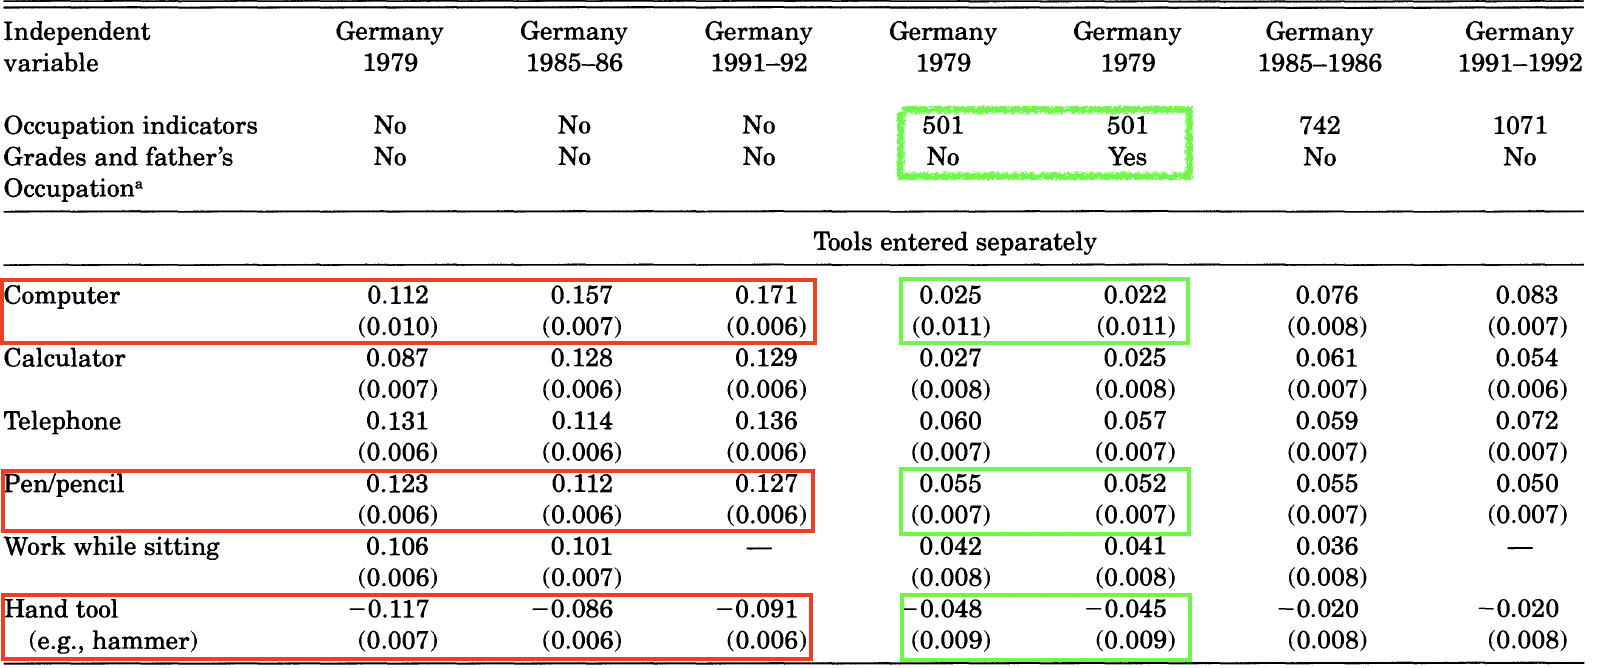
\includegraphics[width=\linewidth]{images/dinardo0.png}
\end{center}
\end{frame}


\begin{frame}{In Practice (2): Exploring the results}
\begin{itemize}
  \item To account for potential selection effects related to occupations, the analysis includes occupation dummy variables.\\[1em]
  \item These occupation dummies help control for variations in wage structures across different jobs.\\[1em]
  \item Even within narrowly defined occupations, significant wage differentials for office tools persist.\\[1em]
  \item Ability controls, such as grades and academic achievements, are included in the analysis to address potential selection effects.\\[1em]
  \item Results suggest that ability controls are not proxies for the skills relevant in the workplace.\\[1em]
  \item This indicates that the estimated wage differentials for tools, even within narrowly defined occupations, are not solely due to the workers' academic abilities.\\[1em]
  \item[$\rightarrow$] Strong selection effects seem to persist.
\end{itemize}
\end{frame}


\end{document}